\chapter{Erprobung und Evaluation}
\section{Erprobung durch die Zielgruppe}
\section{Analyse der Erprobungsresultate}
\section{Ableitung von Optimierungsmaßnahmen}
David
% Die Zeitplanung spielt im Kontext des Hochschulprojektes eine bedeutende Rolle,
% da das Projekt zeitlich eng begrenzt und auf zwei verschiedene Semester aufgeteilt ist.
% Es ergibt sich die Notwendigkeit einer detaillierten Planung, um alle Anforderungen
% termingerecht erfüllen zu können und Abhängigkeiten zwischen mehreren Teammitgliedern
% konfliktfrei zu lösen. Weiterhin müssen separate Planungen für die jeweiligen Semester
% durchgeführt werden, da diese zwar abhängig voneinander sind, die Informationen für die
% Planung des höheren Semesters allerdings noch nicht vorhanden sein müssen.

% Die Planung dazu basiert - wie in vorherigen Kapiteln beschrieben - allgemein auf
% festen Abgabeterminen zu bereits festgelegten Meetings. 
% Begonnen wurde mit der groben Definition von Epics
% und Arbeitspakten in Jira, auf deren Basis dann eine vorläufige Planung für beide Semester
% erstellt wurde. Diese konnte schrittweise in ihrem Detailgrad ausgebaut werden.

% Zur Visualisierung wurde die Zeitleiste in Jira verwendet, die einem Gantt-Diagramm ähnelt.
% Das Gantt-Diagramm bietet sich bei der Zeitplanung hierbei besonders an, da es eine
% übersichtliche Möglichkeit bietet, Verknüpfungen mit vorangehenden Vorgängen,
% Dokumentation der Vorgangsverantwortlichen sowie Kapazitätsdarstellungen, in einem
% Diagramm zu veranschaulichen.
% \footcite[Vgl.][123]{osterhageAnhangProjektmanagement2016}
% Dadurch, dass über die Zeitachse Aktivitäten in Form von Balken mit festen Anfangs-
% und Endtermin dargestellt werden, können Abhängigkeiten zwischen Aufgaben und
% Arbeitspaketen hergestellt sowie kritische Stellen in der Planung sichtbar gemacht
% werden.
% \footcite[Vgl.][117]{hobelGABLERBUSINESSWISSENAZ2006}
% Zudem erklärt sich die populäre Nutzung von Gantt-Charts auch dadurch, dass
% sie sowohl den Projektteilnehmern eine übersichtliche Visualisierung des Projektfortschritts
% ermöglichen als auch in der finalen Präsentation der Ergebnisse vor dem Management genutzt
% werden können.
% \footcite[Vgl.][435]{wilsonGanttChartsCentenary2003}
% \begin{figure}[H]
%     \centering
%     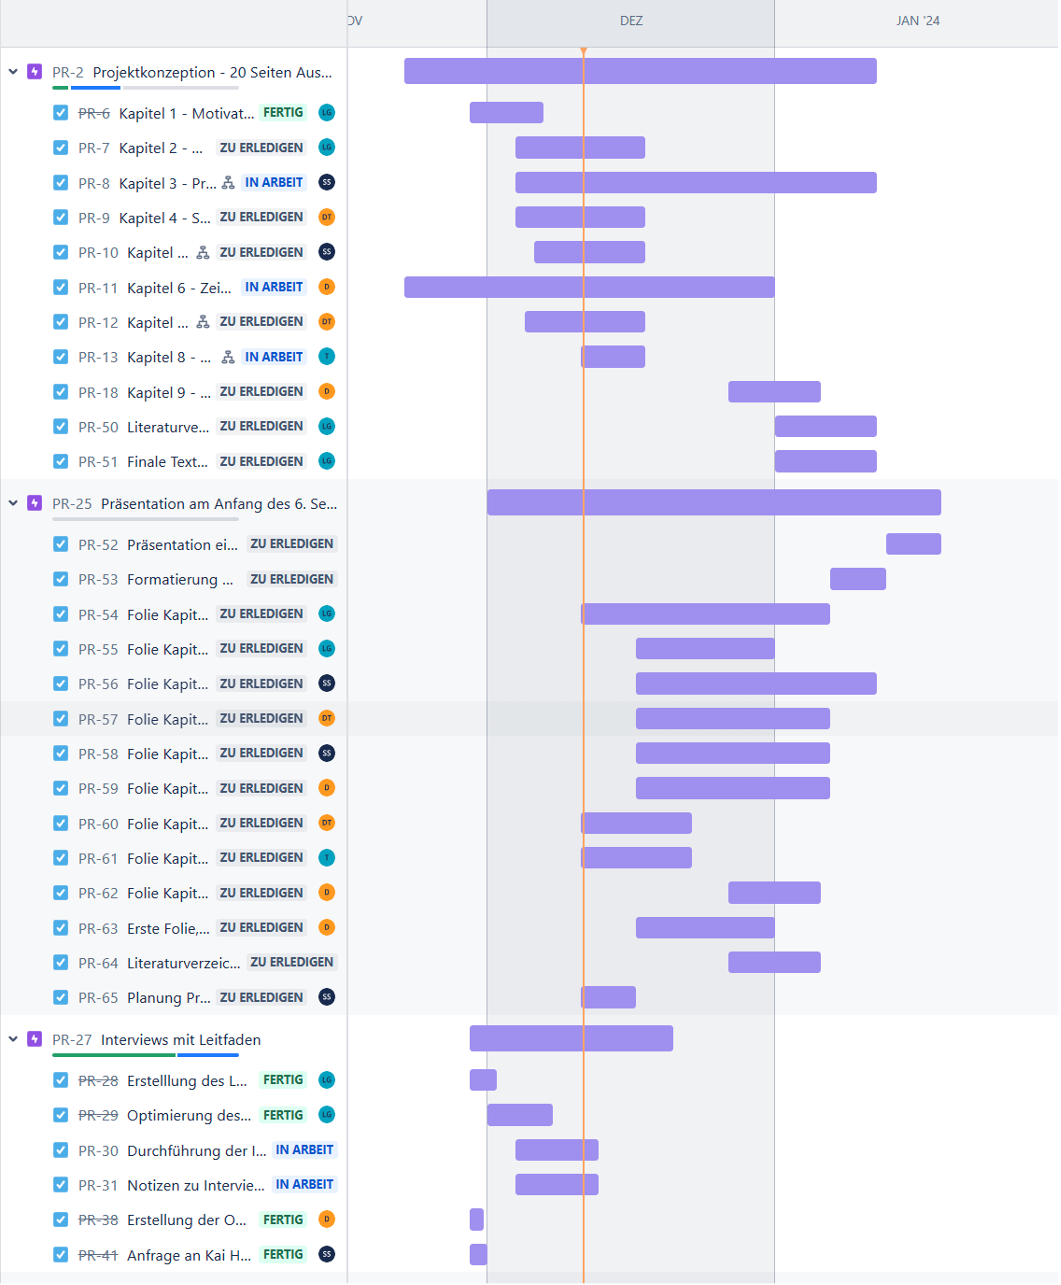
\includegraphics[width=0.9\linewidth]{graphics/zeitplanung.png}
%     \caption{Übersicht über die Zeitplanung in JIRA.}\label{abb:zeitplanung}
% \end{figure}
% Es wird sichtbar, dass die Kapitel nach einer logischen Reihenfolge eingeteilt worden sind.
% Allgemeine Planungsthemen wie Projektplanung oder
% Zeitplanung sind auf einen größeren Zeitraum zugeschnitten, konkrete Kapitelthemen wie die
% Einleitung oder auch die Anforderungen dagegen für kurze und spezifische Zeitperioden vorgesehen
% sowie in einer für den Ablauf effizienten, sequenziellen Reihenfolge angeordnet. Hieraus ergibt
% sich, dass das sechste Semester überwiegend für die Umsetzung genutzt werden kann und jegliche
% Planung bereits zu großen Teilen finalisiert ist.

% Bezüglich der Umsetzungsplanung lässt sich feststellen, dass die Umsetzung der Schulungsunterlage
% einige Abhängigkeiten mit sich bringt. So erfordert sie enge Absprachen mit dem zweiten
% Schulungs-Team, um keine Dopplungen zu erhalten. Diese Planung kann sich jedoch aufgrund
% des neuen Vorlesungsplans im sechsten Semester noch ändern. 

